%% Præsentation for C-programmering for begyndere
%% Lavet af Jacob Bechmann Pedersen og Jacob Skjødt Nielsen
%% For C undervisning i IDA 
%%
%% Theme: `DarkConsole'
%% Copyright (c) 2011-2017 Kazuki Maeda <kmaeda@kmaeda.net>
%% Distributable under the MIT License:
%% http://www.opensource.org/licenses/mit-license.php 

%% Preamble
\documentclass{beamer}

\usepackage{hyperref} % Add a link to your document
\usepackage{graphicx} % Add pictures to your document
\usepackage{listings} % Source code formatting and highlighting
\usepackage[utf8]{inputenc} % Gives UTF-8 encoded characters such as Æ, Ø, Å.

%% Setting the C language type, for viewing pleasure:
\usepackage{listings}
\usepackage{color}

\definecolor{link}{HTML}{CF55E3}
\definecolor{dkgreen}{rgb}{0,0.6,0}
\definecolor{gray}{rgb}{0.5,0.5,0.5}

\lstset{frame=tb,
  inputencoding=utf8,
  language=C,
  aboveskip=3mm,
  belowskip=3mm,
  showstringspaces=false,
  columns=flexible,
  basicstyle={\small\ttfamily},
  numbers=left,
  numbersep=0pt,
  keywordsprefix={\#, \<},
  numberstyle=\tiny\color{gray},
  keywordstyle=\color{C_darkblue},
  commentstyle=\color{dkgreen},
  stringstyle=\color{C_lightblue},
  breaklines=true,
  breakatwhitespace=true,
  tabsize=3,
  extendedchars=true,
  literate={æ}{{\ae}}1 {ø}{{\o}}1 {å}{{\r a}}1 {Æ}{{\AE}}1 {Ø}{{\O}}1 {Å}{{\r A}}1,
}

\usetheme{C_Console}
\title{C-Programmering for begyndere}
\date{16. april 2018}
\subtitle{Del 3 - Funktioner, arrays, datarepræsentationer}
\author{Jacob B. Pedersen\footnote{jacob.bp@mvb.net} og Jakob S. Nielsen\footnote{jakob990@gmail.com}}

%% Document
\begin{document}

\begin{frame}
	\maketitle
\end{frame}

\begin{frame}{Indhold}
	\tableofcontents
\end{frame}

\section{Repetition}
%%----------------------------------------------------------------------
\subsection{Hvad lavede vi sidste gang?}

\begin{frame}[fragile]{Hvad lavede vi sidste gang?}
	\begin{itemize}
		\item{Vi gennemgik operatorer, og deres betydning for if-else statements:}
		\begin{lstlisting}
		if([betingelse]){
			handling();
		}
		else if({betingelse2]){
			handling2();
		}
		else{
			handling3();
		}
		\end{lstlisting}
	\end{itemize}
\end{frame}

%----------------------------------------------------------------------

\begin{frame}[fragile]{Hvad lavede vi sidste gang?}
	\begin{itemize}
		\item{Operatorerne selv evalueredes blot til Boolske udtryk som {\color{dkgreen}true} og {\color{dkgreen}false}:}
		\begin{lstlisting}
		1 > 2; // false
		3 >= 3; // true
		12 > 2 && 12 < 11; // false
		12 > 2 || 12 < 11; // true
		\end{lstlisting}
	\end{itemize}
\end{frame}


%----------------------------------------------------------------------

\begin{frame}[fragile]{Hvad lavede vi sidste gang?}
	\begin{itemize}
		\item{På samme måde kunne de også bruges som betingelser i løkkerne}
		\item{Her var der {\color{C_darkblue}while}() og {\color{C_darkblue}for}() -løkkerne:}
		\begin{lstlisting}
		int i = 0;
		while(i <= 10){
			printf(”%d”, i);
			i++;
		}

		for(int j = 0; j <= 10, j++){
			printf(”%d”, j);
		}
		\end{lstlisting}
	\end{itemize}
\end{frame}

%----------------------------------------------------------------------

\begin{frame}[fragile]{Hvad lavede vi sidste gang?}
	\begin{itemize}
		\item{Til sidst kiggede vi på {\color{C_darkblue}switch}-cases:}
		\begin{lstlisting}
		switch(variabel)
		{
			case 1:
			handling();
			break;

			case 2:
			andenHandling();
			break;

			default:
			break;
		}
		\end{lstlisting}
	\end{itemize}
\end{frame}

\section{I dag}
%%----------------------------------------------------------------------
\subsection{Dagens program}

\begin{frame}[fragile]{Dagens program}
	\begin{itemize}
		\item{I dag kigger vi på mere avanceret brug af C:}
		\item{Funktioner}
		\begin{itemize}
			\item{Genopfriske argumenter og retur-værdier}
			\item{Header- og implementationsfiler}
			\item{Hvad skal der til for at lave et library?}
		\end{itemize}
		\item{Arrays}
		\begin{itemize}
			\item{Lister over variable, refereret til ved indeks}
			\item{Nogle af jer har forsøgt sig med char array AKA strings}
		\end{itemize}
		\item{Anderledes datarepræsentation:}
		\begin{itemize}
			\item{{\color{C_darkblue}typedef} og {\color{C_darkblue}enum}}
			\item{Klynger af data i {\color{C_darkblue}structs}}
			\item{Flerformet data i {\color{C_darkblue}unions}}
		\end{itemize}
	\end{itemize}
\end{frame}

%%----------------------------------------------------------------------
\subsection{Funktioner}

\begin{frame}[fragile]{Funktioner}
	\begin{itemize}
		\item{Vi har ofte brugt funktioner:}
		\begin{itemize}
			\item{{\color{C_darkblue}pow}(), {\color{C_darkblue}sqrt}(), {\color{C_darkblue}rand}(), {\color{C_darkblue}printf}() og {\color{C_darkblue}scanf}()}
		\end{itemize}
		\item{De ligner alle i skrift lidt matematiske funktioner:}
		\begin{equation}
      	printf(x)
    		\end{equation}
    		\item{Og vi kan selvfølgelig også designe vores egne!}
    		\item{Vi husker tydeligt en funktionsdefinition, vi har med hver gang:}
    		\begin{lstlisting}
		int main(int argc, char ** argv){
			return 0;
		}
		\end{lstlisting}
	\end{itemize}
\end{frame}

%%----------------------------------------------------------------------

\begin{frame}[fragile]{Funktioner}
	\begin{itemize}
		\item{I funktionerne er der en række begrber vi skal genopfriske/kende:}
		\begin{itemize}
			\item{{\color{dkgreen}returtype}, {\color{dkgreen}argumenttype/parameter}, {\color{dkgreen}returværdi} og {\color{dkgreen}lokale variable}:}
		\end{itemize}
	\begin{center}
		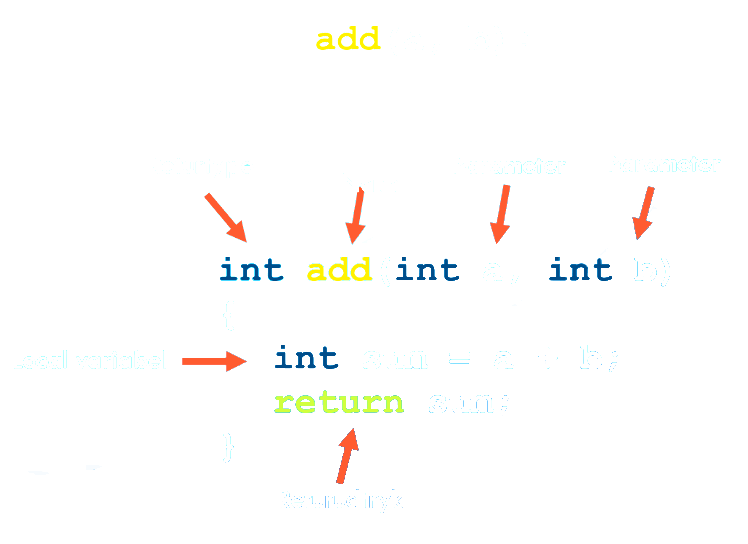
\includegraphics[width=0.7\textwidth]{assets/function_description.png}
	\end{center}
	\end{itemize}
\end{frame}

%%----------------------------------------------------------------------

\begin{frame}[fragile]{Funktioner}
	\begin{itemize}
		\item{Så først defineres funktionen, og derefter  kan den kaldes som alt andet i main:}
		\begin{lstlisting}
		int add( int a, int b ){
			int result = a + b;
			return result;
		}

		int main(void){
			int a = 3;
			int b = 2;
			printf(”%d + %d = %d”, a, b, add(a,b));
		}
		\end{lstlisting}
	\end{itemize}
\end{frame}

%%----------------------------------------------------------------------

\begin{frame}[fragile]{Funktioner}
	\begin{itemize}
		\item{Noget andet fedt man kan med sine funktioner, er at kalde dem rekursivt:}
		\begin{lstlisting}
		int rekursion(int antalGange){
			if(antalGange < 0){
			return 0;
			}
			printf(”%d”, rekursion(antalGange-1));
			return antalGange;
		}
		\end{lstlisting}
	\end{itemize}
\end{frame}

\section{Kreative Opgaver}
%%----------------------------------------------------------------------
\begin{frame}{Kreative Opgaver}
	\begin{itemize}
	\item{Det var det for nu!}
	\item{Der ligger som sidst kreative opgaver tilgængelige:}
		\begin{itemize}
		\item{\color{link}\href{https://github.com/Iakop/C-Programmering-for-begyndere/tree/master/Del_2/Exercises/C_exercises_2_dansk.pdf}{../Del\_2/Exercises/C\_exercises\_2\_dansk.pdf}}
		\end{itemize}
	\item{Der er hjælp at hente her på workshoppen}
	\item{God arbejdslyst! - Happy Hacking!}
	\end{itemize}
\end{frame}



\end{document}

%%\begin{frame}[fragile]
	%%\begin{lstlisting}
		%%#include <stdio.h>

		%%int main(void)
		%%{
		%%printf("Hello world\n");
		%%return 0;
		%%}
	%%\end{lstlisting}
%%\end{frame}